\documentclass[12pt,addpoints]{exam}
%\usepackage{enumitem}
\usepackage{amsfonts,amssymb,amsmath, amsthm}
\usepackage{graphicx}
\usepackage{systeme}
\usepackage{pgf,tikz,pgfplots}
\pgfplotsset{compat=1.15}
\usepgfplotslibrary{fillbetween}
\usepackage{mathrsfs}
\usetikzlibrary{arrows}
\usetikzlibrary{calc}
\usepackage{geometry}
\geometry{
	a4paper,
	total={170mm,257mm},
	left=20mm,
	top=15mm,
}
\pagestyle{headandfoot}
%\firstpageheadrule
\runningheader{Two Dimensional Motion}{}{Page \thepage\ of \numpages}
\runningheadrule
\firstpagefooter{}{}{}
\runningfooter{By Aaron G.K.}{}{Page \thepage\ of \numpages}
\title{Two Dimensional Motion}
\author{Aaron G.K.}
\begin{document}
	\maketitle
	\begin{center}
		\subsection*{Modeling 2D Motion}
	\end{center}
	We have introduced the concepts of position, velocity and acceleration to describe motion in one dimension; however we live in a multidimensional universe. \\ \\
	To do that, we must extend our definitions of position, velocity, and acceleration for an object that moves in two dimensions by treating each direction independently, which we can do with vector quantities by resolving each of these quantities into their components defined by the basis vectors. For example, our definition of velocity as the derivative of position holds for each component separately. In Cartesian coordinates, the position vector $\vec r(t)$ with respect to some choice of origin for the object at time t is given by
	$$\overrightarrow{\mathbf{r}}(t)=x(t) \hat{\mathbf{i}}+y(t) \hat{\mathbf{j}}$$
	The velocity vector $\vec v(t)$ at time t is the derivative of the position vector, 
	$$\overrightarrow{\mathbf{v}}(t)=\frac{d x(t)}{d t} \hat{\mathbf{i}}+\frac{d y(t)}{d t} \hat{\mathbf{j}} = v_{x}(t) \hat{\mathbf{i}}+v_{y}(t) \hat{\mathbf{j}} \nonumber$$
	where $v_{x}(t) =\dfrac{dx(t)}{dt}$ and $v_{y}(t) = \dfrac{dy(t)}{dt}$ denote the x - and y -components of the velocity respectively.
	The acceleration vector $\vec a(t)$ is defined in a similar fashion as the derivative of the velocity vector,
	$$\overrightarrow{\mathbf{a}}(t)=\frac{d v_{x}(t)}{d t} \hat{\mathbf{i}}+\frac{d v_{y}(t)}{d t} \hat{\mathbf{j}} = a_{x}(t) \hat{\mathbf{i}}+a_{y}(t) \hat{\mathbf{j}}$$
	where $a_x(t)=\dfrac{dv_x(t)}{dt}$ and $a_y(t)=\dfrac{dv_y(t)}{dt}$ denote the x- and y-components of the acceleration. \\ \\
	The natural way we should start two dimensional motion should be projectile motion. However, we have discussed projectile motion last year and redundancy would not suffice, hence we will be moving forward with the next common topic in 2D motion, which is circular motion.
	\subsection*{Circular Motion}
	A special class of motions, motion in a plane about a central point, a motion we shall refer to as \textbf{central motion}, the most outstanding case of which is \textbf{circular motion}. \\ \\
	Let's begin by describing the kinematics of circular motion. We see that unlike linear motion, where velocity and acceleration are directed along the line of motion, in circular motion the direction of velocity is always tangent to the circle. This means that as the object moves in a circle, the direction of the velocity is always changing. We also see that the direction of the change of the velocity is towards the center of the circle. This means that there is a non-zero component of the acceleration directed radially inward, which is called the centripetal acceleration. If our object is increasing its speed or slowing down, there is also a non-zero tangential acceleration in the direction of motion. But when the object is moving at a constant speed in a circle then only the centripetal acceleration is non-zero.\\ \\
	Twenty years before Newton published Principia Mathematica, he realized that the moon is always “falling” towards the center of the earth; otherwise, by the First Law, it would continue in some linear trajectory rather than follow a circular orbit. Therefore there must be a centripetal force, a radial force pointing inward, producing this centripetal acceleration. \\ \\
	When an object is constrained to move in a circle, there must exist a force $\vec{F}$ acting on the object directed towards the center. Because Newton’s Second Law is a vector equality, the radial component of the Second Law is
	$$F_{r}=m a_{r} \nonumber$$
	Let's start with the kinematics of circular motion. We begin our description of circular motion by choosing polar coordinates(\textit{because they are obviously much better in this sense}). In the figure below we sketch the position vector $\vec{r(t)}$ of the object moving in a circular orbit of radius r.
	\begin{center}
		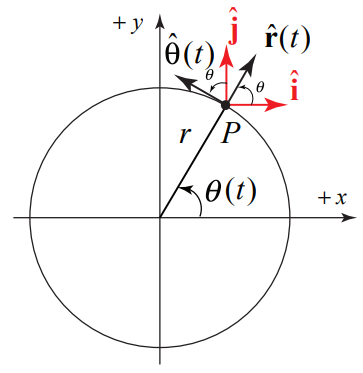
\includegraphics[scale=0.4]{circ.png}
	\end{center}
	At time $t$, the particle is located at the point P with coordinates  $(r,\theta(t))$ and position vector given by
	$$\overrightarrow{\mathbf{r}}(t)=r \hat{\mathbf{r}}(t)$$
	At the point P, consider two sets of unit vectors ($\hat{r}(t)$, $\hat{\theta}(t)$) and ($\hat{i}$, $\hat{j}$), as shown in the figure above. The vector decomposition expression for $\hat{r}(t)$ and $\hat{\theta}(t)$ in terms of $\hat{i}$ and $\hat{j}$ is given by
	$$\hat{\mathbf{r}}(t)=\cos \theta(t) \hat{\mathbf{i}}+\sin \theta(t) \hat{\mathbf{j}}$$
	$$\hat{\boldsymbol{\theta}}(t)=-\sin \theta(t) \hat{\mathbf{i}}+\cos \theta(t) \hat{\mathbf{j}}$$
	To calculate the velocities, we should compute the derivative of the functions above. For the first one($\vec{\mathbf{v}}(t)=\dfrac{d\vec{r}(t)}{dt}$),
	$$\begin{array}{l} 
		\frac{d \hat{\mathbf{r}}(t)}{d t}=\frac{d}{d t}(\cos \theta(t) \hat{\mathbf{i}}+\sin \theta(t) \hat{\mathbf{j}})=\left(-\sin \theta(t) \frac{d \theta(t)}{d t} \hat{\mathbf{i}}+\cos \theta(t) \frac{d \theta(t)}{d t} \hat{\mathbf{j}}\right) \\ 
		=\frac{d \theta(t)}{d t}(-\sin \theta(t) \hat{\mathbf{i}}+\cos \theta(t) \hat{\mathbf{j}})=\frac{d \theta(t)}{d t} \hat{\mathbf{\theta}}(t) 
	\end{array} \nonumber$$
	For the second vector, which is $\vec{\boldsymbol{\omega}}=\dfrac{d\hat{\boldsymbol{\theta}}(t)}{dt}$,
	$$\begin{array}{l} 
		\frac{d \hat{\boldsymbol{\theta}}(t)}{d t}=\frac{d}{d t}\left(-\sin \theta(t) \hat{\mathbf{i}}+\cos \theta(t \hat{\mathbf{j}})=\left(-\cos \theta(t) \frac{d \theta(t)}{d t} \hat{\mathbf{i}}-\sin (t) \frac{d \theta(t)}{d t} \hat{\mathbf{j}}\right)\right. \\ 
		=\frac{d \theta(t)}{d t}(-\cos \theta(t) \hat{\mathbf{i}}-\sin \theta(t) \hat{\mathbf{j}})=-\frac{d \theta(t)}{d t} \hat{\mathbf{r}}(t) 
	\end{array} \nonumber$$
	From the above relationship, we get the following expression below which gives us the velocity vector,
	$$\overrightarrow{\mathbf{v}}(t)=\frac{d \overrightarrow{\mathbf{r}}(t)}{d t}=r \frac{d \hat{\mathbf{r}}}{d t}=r \frac{d \theta}{d t} \hat{\boldsymbol{\theta}}(t)=v_{\theta} \hat{\boldsymbol{\theta}}(t) \nonumber$$
	where the  $\hat{\boldsymbol{\theta}}$-component of the velocity is given by
	$$v_{\theta}=r \frac{d \theta}{d t} \nonumber$$
	$\vec{v}(t)$ is referred to as the tangential component of the velocity. Denote the magnitude of the velocity by  $v=|\vec{v}|$. The angular speed is the magnitude of the rate of change of angle with respect to time, which we denote by the Greek letter $\omega$,
	$$\omega \equiv\left|\frac{d \theta}{d t}\right| \nonumber$$
	We can also geometrically derive the equations above which are left for you, the readers aka the students :).
\end{document}	